% Neural network diagram
% Made with Xematics. Positions are in px (1 px = 0.75 pt), as in the SVG export.
\documentclass[tikz, border=4pt]{standalone}
\usetikzlibrary{arrows.meta}
\definecolor{xm1}{HTML}{FFFFFF}
\definecolor{xm2}{HTML}{6B7280}
\definecolor{xm3}{HTML}{D4E8F5}
\definecolor{xm4}{HTML}{0072B2}
\definecolor{xm5}{HTML}{F1F2F4}
\definecolor{xm6}{HTML}{4B5563}
\definecolor{xm7}{HTML}{DFE3E8}
\definecolor{xm8}{HTML}{FBE8C4}
\definecolor{xm9}{HTML}{B97800}
\definecolor{xm10}{HTML}{AEB3B9}
\definecolor{xm11}{HTML}{1F2937}
\begin{document}
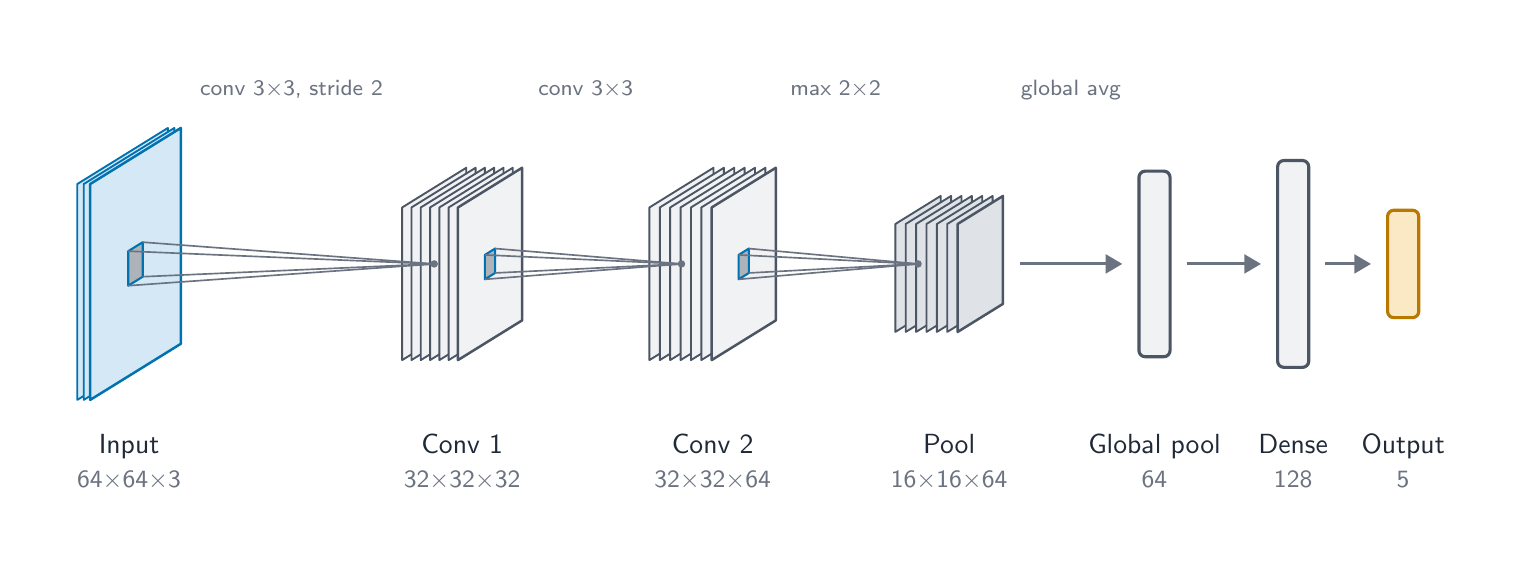
\begin{tikzpicture}[x=0.75pt, y=-0.75pt]
  \tikzset{
    xm arrow/.style={draw=xm2, line width=1.05pt, -{Triangle[length=6pt, width=6.75pt]}},
    xm map input back/.style={fill=xm3, draw=xm4, line width=0.68pt, line join=round},
    xm map input/.style={fill=xm3, draw=xm4, line width=0.9pt, line join=round},
    xm map hidden back/.style={fill=xm5, draw=xm6, line width=0.68pt, line join=round},
    xm map hidden/.style={fill=xm5, draw=xm6, line width=0.9pt, line join=round},
    xm map pool back/.style={fill=xm7, draw=xm6, line width=0.68pt, line join=round},
    xm map pool/.style={fill=xm7, draw=xm6, line width=0.9pt, line join=round},
    xm box hidden/.style={fill=xm5, draw=xm6, line width=1.13pt, rounded corners=2.25pt},
    xm box output/.style={fill=xm8, draw=xm9, line width=1.13pt, rounded corners=2.25pt},
    xm window/.style={fill=xm10, draw=xm4, line width=0.75pt, line join=round},
    xm ray/.style={draw=xm2, line width=0.6pt},
    xm ray end/.style={fill=xm2},
    xm name xm11/.style={text=xm11, inner sep=0, font=\sffamily\fontsize{9.75}{11.7}\selectfont},
    xm size xm2/.style={text=xm2, inner sep=0, font=\sffamily\fontsize{9}{10.8}\selectfont},
    xm op xm2/.style={text=xm2, inner sep=0, font=\sffamily\fontsize{8.25}{9.9}\selectfont},
  }
  \fill[xm1] (0,0) rectangle (705.94,246.6);
  % Connections 3
  \draw[xm arrow] (477.89,113.83) -- (527.4,113.83);
  % Connections 4
  \draw[xm arrow] (558.4,113.83) -- (594.21,113.83);
  % Connections 5
  \draw[xm arrow] (625.21,113.83) -- (647.2,113.83);
  % Layers
  \draw[xm map input back] (23.89,75.35) -- (67.57,48.31) -- (67.57,152.31) -- (23.89,179.35) -- cycle;
  \draw[xm map input back] (27,75.35) -- (70.68,48.31) -- (70.68,152.31) -- (27,179.35) -- cycle;
  \draw[xm map input] (30.11,75.35) -- (73.79,48.31) -- (73.79,152.31) -- (30.11,179.35) -- cycle;
  \draw[xm map hidden back] (180.43,86.62) -- (211.32,67.5) -- (211.32,141.04) -- (180.43,160.16) -- cycle;
  \draw[xm map hidden back] (184.91,86.62) -- (215.8,67.5) -- (215.8,141.04) -- (184.91,160.16) -- cycle;
  \draw[xm map hidden back] (189.39,86.62) -- (220.28,67.5) -- (220.28,141.04) -- (189.39,160.16) -- cycle;
  \draw[xm map hidden back] (193.87,86.62) -- (224.76,67.5) -- (224.76,141.04) -- (193.87,160.16) -- cycle;
  \draw[xm map hidden back] (198.35,86.62) -- (229.24,67.5) -- (229.24,141.04) -- (198.35,160.16) -- cycle;
  \draw[xm map hidden back] (202.83,86.62) -- (233.72,67.5) -- (233.72,141.04) -- (202.83,160.16) -- cycle;
  \draw[xm map hidden] (207.31,86.62) -- (238.19,67.5) -- (238.19,141.04) -- (207.31,160.16) -- cycle;
  \draw[xm map hidden back] (299.56,86.62) -- (330.44,67.5) -- (330.44,141.04) -- (299.56,160.16) -- cycle;
  \draw[xm map hidden back] (304.56,86.62) -- (335.44,67.5) -- (335.44,141.04) -- (304.56,160.16) -- cycle;
  \draw[xm map hidden back] (309.56,86.62) -- (340.44,67.5) -- (340.44,141.04) -- (309.56,160.16) -- cycle;
  \draw[xm map hidden back] (314.56,86.62) -- (345.44,67.5) -- (345.44,141.04) -- (314.56,160.16) -- cycle;
  \draw[xm map hidden back] (319.56,86.62) -- (350.44,67.5) -- (350.44,141.04) -- (319.56,160.16) -- cycle;
  \draw[xm map hidden back] (324.56,86.62) -- (355.44,67.5) -- (355.44,141.04) -- (324.56,160.16) -- cycle;
  \draw[xm map hidden] (329.56,86.62) -- (360.44,67.5) -- (360.44,141.04) -- (329.56,160.16) -- cycle;
  \draw[xm map pool back] (418.05,94.59) -- (439.89,81.07) -- (439.89,133.07) -- (418.05,146.59) -- cycle;
  \draw[xm map pool back] (423.05,94.59) -- (444.89,81.07) -- (444.89,133.07) -- (423.05,146.59) -- cycle;
  \draw[xm map pool back] (428.05,94.59) -- (449.89,81.07) -- (449.89,133.07) -- (428.05,146.59) -- cycle;
  \draw[xm map pool back] (433.05,94.59) -- (454.89,81.07) -- (454.89,133.07) -- (433.05,146.59) -- cycle;
  \draw[xm map pool back] (438.05,94.59) -- (459.89,81.07) -- (459.89,133.07) -- (438.05,146.59) -- cycle;
  \draw[xm map pool back] (443.05,94.59) -- (464.89,81.07) -- (464.89,133.07) -- (443.05,146.59) -- cycle;
  \draw[xm map pool] (448.05,94.59) -- (469.89,81.07) -- (469.89,133.07) -- (448.05,146.59) -- cycle;
  \draw[xm box hidden] (535.4,69.12) rectangle ++(15,89.41);
  \draw[xm box hidden] (602.21,64.01) rectangle ++(15,99.65);
  \draw[xm box output] (655.2,87.95) rectangle ++(15,51.76);
  \draw[xm window] (48.45,107.67) -- (55.44,103.35) -- (55.44,119.99) -- (48.45,124.31) -- cycle;
  \draw[xm ray] (48.45,107.67) -- (195.87,113.83);
  \draw[xm ray] (55.44,103.35) -- (195.87,113.83);
  \draw[xm ray] (55.44,119.99) -- (195.87,113.83);
  \draw[xm ray] (48.45,124.31) -- (195.87,113.83);
  \fill[xm ray end] (195.87,113.83) circle[radius=1.8];
  \draw[xm window] (220.28,109.48) -- (225.22,106.42) -- (225.22,118.18) -- (220.28,121.24) -- cycle;
  \draw[xm ray] (220.28,109.48) -- (315,113.83);
  \draw[xm ray] (225.22,106.42) -- (315,113.83);
  \draw[xm ray] (225.22,118.18) -- (315,113.83);
  \draw[xm ray] (220.28,121.24) -- (315,113.83);
  \fill[xm ray end] (315,113.83) circle[radius=1.8];
  \draw[xm window] (342.53,109.48) -- (347.47,106.42) -- (347.47,118.18) -- (342.53,121.24) -- cycle;
  \draw[xm ray] (342.53,109.48) -- (428.97,113.83);
  \draw[xm ray] (347.47,106.42) -- (428.97,113.83);
  \draw[xm ray] (347.47,118.18) -- (428.97,113.83);
  \draw[xm ray] (342.53,121.24) -- (428.97,113.83);
  \fill[xm ray end] (428.97,113.83) circle[radius=1.8];
  % Labels
  \node[xm name xm11, anchor=base] at (48.84,204.94) {Input};
  \node[xm size xm2, anchor=base] at (48.84,221.7) {64\ensuremath{\times}64\ensuremath{\times}3};
  \node[xm op xm2, anchor=base] at (127.11,32.66) {conv 3\ensuremath{\times}3, stride 2};
  \node[xm name xm11, anchor=base] at (209.31,204.94) {Conv 1};
  \node[xm size xm2, anchor=base] at (209.31,221.7) {32\ensuremath{\times}32\ensuremath{\times}32};
  \node[xm op xm2, anchor=base] at (268.88,32.66) {conv 3\ensuremath{\times}3};
  \node[xm name xm11, anchor=base] at (330,204.94) {Conv 2};
  \node[xm size xm2, anchor=base] at (330,221.7) {32\ensuremath{\times}32\ensuremath{\times}64};
  \node[xm op xm2, anchor=base] at (389.24,32.66) {max 2\ensuremath{\times}2};
  \node[xm name xm11, anchor=base] at (443.97,204.94) {Pool};
  \node[xm size xm2, anchor=base] at (443.97,221.7) {16\ensuremath{\times}16\ensuremath{\times}64};
  \node[xm op xm2, anchor=base] at (502.64,32.66) {global avg};
  \node[xm name xm11, anchor=base] at (542.9,204.94) {Global pool};
  \node[xm size xm2, anchor=base] at (542.9,221.7) {64};
  \node[xm name xm11, anchor=base] at (609.71,204.94) {Dense};
  \node[xm size xm2, anchor=base] at (609.71,221.7) {128};
  \node[xm name xm11, anchor=base] at (662.7,204.94) {Output};
  \node[xm size xm2, anchor=base] at (662.7,221.7) {5};
\end{tikzpicture}
\end{document}
